\documentclass[12pt, letterpaper]{article}
\usepackage[utf8]{inputenc}
\usepackage{graphicx}
\usepackage{hyperref}

\title{Rapport personnel pour le cours de compréhension de programme}
\author{Chaolei CAI \ 17812776}

\begin{document}


\begin{titlepage}
    \maketitle
\end{titlepage}

\tableofcontents
\section{Introduction}
Ce document est le rapport personnel de CAI Chaolei pour le cours compréhension de programme\\
Je suis dans le groupe 1 avec Ramu Danabal, Omar Hammouche, Predrag Kostic et Komlan Dantodji. \\
Notre projet portait sur l'outil Gimp, plus précisement la version 2.10.14\\
L'environnement de test et d'utilisation est la distribution Linux : Manjaro-XFCE 64bit 18.1.3\\
Un dépôt GitHub a été crée pour ce projet, il peut être consulté depuis ce lien \url{https://github.com/pkostic-git/gimp-2-10-12-p8}


\section{Objectives}
1/Modification de la boîte à outils, plus précisement de l'outil "Text", il faut le modifier afin qu'il affiche "groupe 1 text" au lieu de "Text."\\
2/Modifier la police et la taille de la police de defaut.\\
3/Ajouter un nouveau 'outil' ou 'boutton' qui change la taille de la police utilisée par une autre taille.\\
4/Ajouter un nouveau 'outil' ou 'boutton' qui ouvriras une fênetre de dialog qui afficheras le résultat de la commande "ls -l" depuis le répertoire courant.

\section{Démarrage du projet}
Au début, le groupe a choisit de mettre l'accent sur la recherche car la machine virtuelle de test n'était pas encore mise en place, j'ai commencé à régler ma machine virtuelle sur la distribution Ubuntu 18.04LTS.\\
Je me suis porté volontaire pour mettre en place la machine virtuelle car c'était un peu compliqué pour les autres de l'installer. Ils se sont donc misent à faire des recherches sur les objectives sur internet.
 Maleuheusement, il n'y a pas vraiment de sujet ou de tutoriel sur internet qui nous apprends à customiser gimp. Il y'a certe le wiki de Gimp mais cela ne fut pas d'une grande aide.\\


\section{Compilation}
Il y avait un problème de version très pénible avec Ubuntu quand j'avais essayé de compiler les codes sources, en effet cela est due au gestionnaire de paquet d'Ubuntu qui ne dispose pas des dernières versions des bibliothèques demandées par Gimp.\\
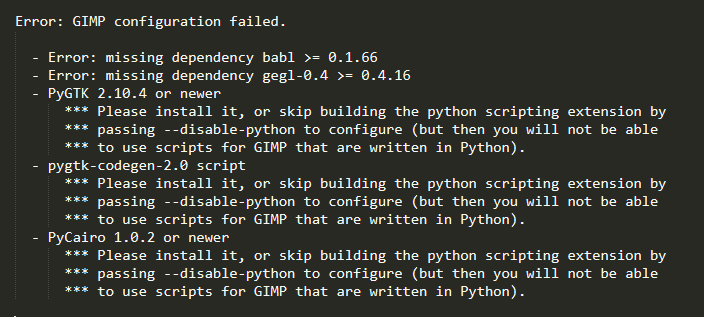
\includegraphics[width=\linewidth]{c1.png}
J'ai crée dans le dépot un fichier DEPENDENCIES.txt dans le répertoire gimp-2.10.12/ , il contient tous les noms de paquet que j'ai pu installé sur la machine.\\
Le problème était que Gimp requière les bibliothèque babl et gegl, mais apt ne disposait que des versions anciennes.
J'ai due donc télecharger le code source pour babl et gegl afin de les installer manuellement, et là je suis tombé dans le piège infernal des dépendances de paquet, l'un d'entre eux demandait svg, ninja et meso. Comme d'habitude apt ne satisfait pas les exigences de versions nécessaire, encore un fois il fallait compiler le code source manuellement... De nouvelles dépendences etc.\\
Finalement, le problème fut réglé en changeant de distribution, je suis donc passé à la distribution Manjaro, ce dernier utilisait pacman comme gestionnaire de paquet. J'ai beaucoup plus d'habitude avec pacman que apt comme j'utilise Arch Linux qui a le même gestionnaire de paquet. Plus besoin de se casser la tête pour les versions car pacman propose toujours la version la plus récente sauf indication de l'utilisateur.
C'est ainsi que Gimp compilait et je pu enfin installer l'application.

\section{Proposition d'hypothèse et vérification}
Nous nous somme basé sur ce que nous avons fait dans l'exercice précedent, en repassant à la vue tous les répertoires, nous avons décidé de se concentrer sur le répertoire app/tools et app/code car app contenait le code source de Gimp, tools a probablement un lien proche avec la boîte à outils et core contenait des fonctions primaires de Gimp.\\
La recherche n'était pas fructueuse car la recherche n'était pas assez spécifique, par exemple un grep avec le mot clé "Text" donnait énormément de résultat même en précisant l'option "\$" pour indiquer la fin de ligne.
Néanmoins, nous avons pu trouver le macro qui définissait la police de défaut utilisé par Gimp, il se trouve dans le fichier app/config/gimpcoreconfig.c ligne 60\\
\#define GIMP\_DEFAULT\_FONT          "Sans-serif"\\
Nous avons pu modifier la police de défaut à Inconsolata Bold.\\ \\
Enfin Ramu a trouvé dans le fichier app/tools/gimptextoptions.c la fonction GIMP\_CONFIG\_PROP\_DOUBLE qui permet de modifier la taille de la police de defaut. (ligne 35-40)\\
GIMP\_CONFIG\_PROP\_DOUBLE (object\_class, PROP\_FONT\_SIZE,\\
                     "font-size",\\
                     \_("Font size"),\\
                     \_("Font size"),\\
                     0.0, 8192.0, 62.0,\\
                     GIMP\_PARAM\_STATIC\_STRINGS);\\
En changeant "62.0" à "42" par exemple, la taille de la police a pu être changé.\\
Malgré ces avancés, cela m'a parrue bizarre que nous trouvons l'objective 2 avant l'objective 1, je me suis dit qu'il faut changer la méthode de recherche, ce n'est pas réaliste de passer au crible tous les fichiers de code source de Gimp. Comme le Gimp que j'ai installé était en fraçais, en laissant le curseur sur l'icon de certains outils, on peut y voir afficher une aide "Outil text: créé ou modifie des calques de texte". \\
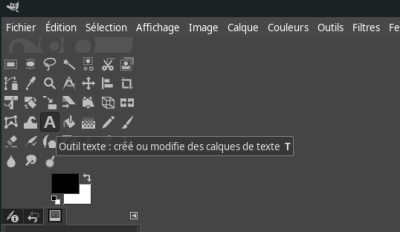
\includegraphics[width=\linewidth]{c2.png}\\
J'ai donc effectué un grep sur cette phrase. Sans surprise, il mène directement vers le répertoire po/ qui contient la traduction vers différents langages. En réduisant ainsi ma recherche sur le fichier "fr.po" j'ai pu trouvé dans ce fichier vers la ligne 23667 ces lignes: \\
\#: ../app/tools/gimptexttool.c:214\\
msgid "Text"\\
msgstr "Texte"\\
Il suffit alors de modifier la ligne "msgstr" de ce fichier pour avoir une affichage modifié. Cependant j'appelle cette modification "locale" car il n'affecte que les utilisateurs dont le langage d'affichage est le français, pour avoir une modification "globale" peu importe la langue utilisée, il faudra aller dans le fichier app/tools/gimptexttool.c ligne 214 et modifier "Text" par l'affichage souhaitée.\\
Nous n'avons pas réussi à ajouter un nouveau boutton dans la boîte à outils, cela étant dit, je pense qu'il faut certainement modifier le fichier app/tools/gimp-tools.c car c'est dans ce fichier qu'il y a une inclusion de headers des outils. J'ai tenté de crée une copie de gimptexttool.c en renommant en mytools.c et en incluant le header mytools.h. C'était un peu trop simple pour que cela fonctionne. nous avons testé d'autre hypothèse comme libgimp/gimpselectbutton.c, libgimp/gimpfontselectbutton.c ou encore \\app/widgets/gimptexteditor.c.
Sans succès, nous nous sommes donc arrêtés jusqu'à cette étape.

\end{document}
